\chapter{Background and related work} \label{background}

In this chapter I describe different types of simulators and the tradeoff between them.
Excellent overviews of the entire field have been written over the years \cite{fujimoto_parallel_2001} \cite{fujimoto_computational_2017} and provide significantly further details on simulation techniques.

\section{Centralized discrete event simulators} \label{centralized-sim}

Event driven simulators typically consist of multiple actors and a scheduler, sometimes referred to as the event queue.
The scheduler is the driver of the simulation, its operation is fairly straightforward: execute the next event, insert any new events at an appropriate place in the queue, launch the next event.
The relatively simple nature of the scheduler makes it so that it can usually be implemented in relatively few lines of code.
\manya{At this point in the thesis, your reader does not know that you implemented multiple simulators and one of them is sequential. please give necessary information to the reader before talking about RotorSim.}
For the sequential simulator, RotorSim\cite{brode-roger_nibriviarotorsim_2020} described in \S \ref{rotorsim}, the loop and event processing code takes up around 30 lines of python.

% not happy with this paragraph structure
\manya{suggestion to make the following para better: start with the goal of this thesis is to simulate a large-scale data center. Then talk about prior papers and available code and cite them as the state of the art for large-scale data center simulations. then talk about millions of events and challenges associated with it......note that, in essence, the closest prior work to your thesis are data center simulators and they need to be discussed in the background section.}
Large simulation models can generate millions or billions of events through their lifetime, if not every second \cite{fujimoto_parallel_2015}, causing the queue to continuously hold thousands or more events at a time, see the results section \S\ref{results} for more details.\manya{Call out a major result from your results section here (and in intro too): For instance, our evaluations in Section X shows that the state-of-the-art Opera \cite{} simulator takes X hours to simulate a network with X servers. In contrast, the simulator developed in this thesis, RustaSim (described in Section X), simulates the same network in only X minutes. }
In addition, since events are typically fast to process, the queue is also continuously being accessed and modified and can easily become a bottleneck.
The large size and frequent access of the queue, force careful consideration of the data structures used to implement the queue.

The queue has to support two operations: retrieving the smallest element currently in the queue, and inserting new events.
This naturally leads to using a min-heap, allowing for $O\left(\log n\right)$ insertion and removal of the smallest element.
Although there exists slightly faster "monotonic heaps", such as the Ladder Queue \cite{tang_ladder_2005}, that are able to further either the complexity or the constant factor, they are usually complex to implement and tune \cite{furfaro_adaptive_2018}, and don't have available efficient implementations. \manya{it's not clear why you are talking about data structures here. If that's the most common data structure in prior simulators, a better flow of the story would be to start with mentioning those simulators and then going deep into their choice of data structure.}
Standard heaps however are common enough that most every language has a well-optimized implementation, often making them easier to use. 

Fundamentally, these simulations are centralized: the scheduler drives the model forward.
Some parallelization is possible if many events are scheduled at the same virtual time and the actors are able to deal with that.
Even if the simulation has many events executing in parallel, we run into issues when they \manya{unclear what "they" refers to, please reword.} try to schedule new events: the scheduler needs to manage multiple new events being enqueued concurrently.
In my experience, the overhead of managing these concurrent operations results in worse performance overall. \manya{please quantify. this is a research thesis, it's not enough to say you experienced worse performance. put it into perspective by giving a more concrete description with numbers}

\manya{is centralized discrete event simulator == single threaded simulator aka all prior data center simulators? if so, it's worth to call it out in this section. if not, mention how they differ.}

\manya{the flow of this section is confusing. Why are you mentioning what is required from the queue? give a roadmap to the reader but telling them what you are going to tell them at the beginning of each subsection. For instance, something line this: in this section I describe the fundamentals of centralized simulators. I identify three? factors as their main bottlenecks: 1) 2) 3) [corresponding to your paragraphs and the main points you are making]...}

\manya{most important missing piece: related work to your thesis (data center simulators) that uses centralized approach.}


\paragraph{Preservation of causality}

In order for a simulation to be correct, it is essential that before any event is processed, all past events it depends on have taken effect.
The dependency on these prior events may be obvious: a packet needs to arrive at a router before it can be sent from said router, or not: in order to know where in the queue to place the arriving packet, it is necessary to know \emph{every} other arriving packet, even if it is from a different source and to a different destination, a previous packet may fill up the router's available memory.

The centralized simulator ensures causality by processing events in absolute time order: by the time any event is executed, all events in its past have fully completed.
Events happening simultaneously are typically assumed to not affect each other and can therefore happen in any order.

\paragraph{Guarantee of progress}
This simulator will always make progress as long as there is another event to process, trivially allowing it to keep making progress until there is none left.



\section{Parallel discrete event simulators} \label{pdes}

The main difficulty in making event simulators parallel lies in guaranteeing causality and progress. \manya{this is a good point to bring in the intro of the thesis.}
It is often easy to guarantee one without the other: without preserving causality, we can process events out of order, and without a need for progress, we are free to advance until it becomes too difficult, and stop then.
Clearly, neither of these solutions are satisfying.

I will describe first the opportunities for concurrency in distributed simulations, then focus on the issues that are raised by needing to make progress.

\subsection{Causality preservation} \label{causality}

\begin{figure}
    \centering
    \begin{subfigure}[t]{0.45\textwidth}
        \centering
        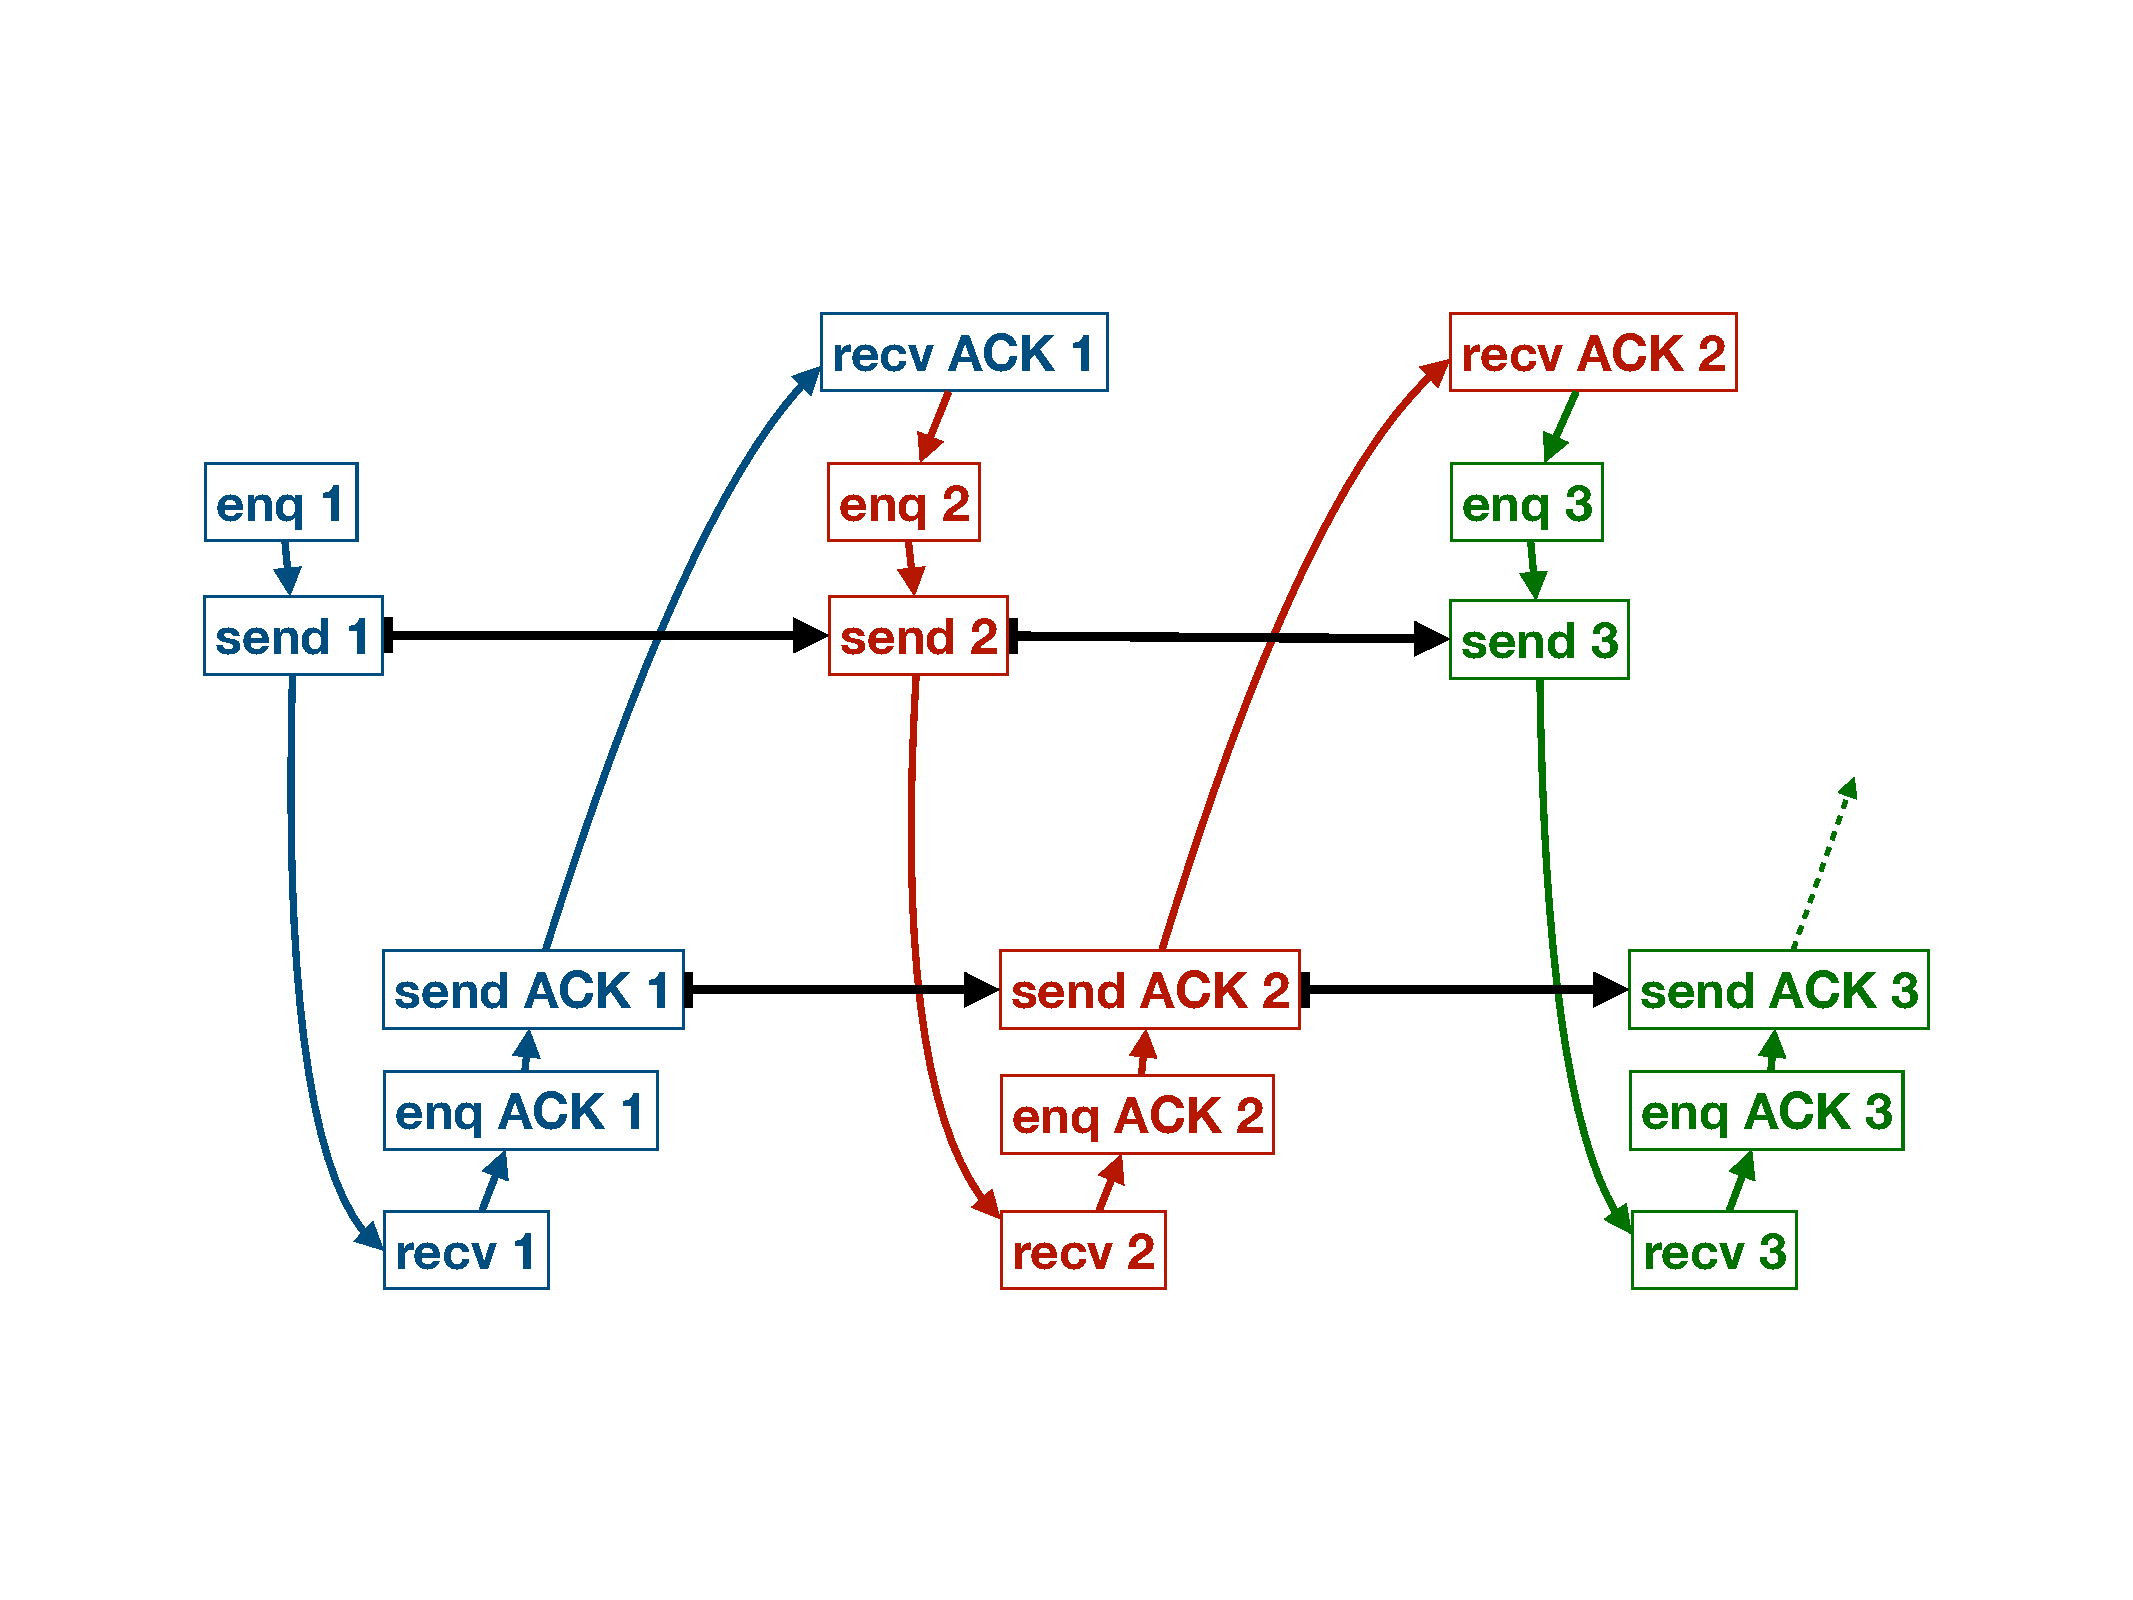
\includegraphics[width=\textwidth]{causality-single}
        \caption{
            This series of events has no opportunity for concurrency: every event directly depends on the previous one.
        }
        \label{causality-graph-seq:fig}
    \end{subfigure}
    \begin{subfigure}[t]{0.45\textwidth}
        \centering
        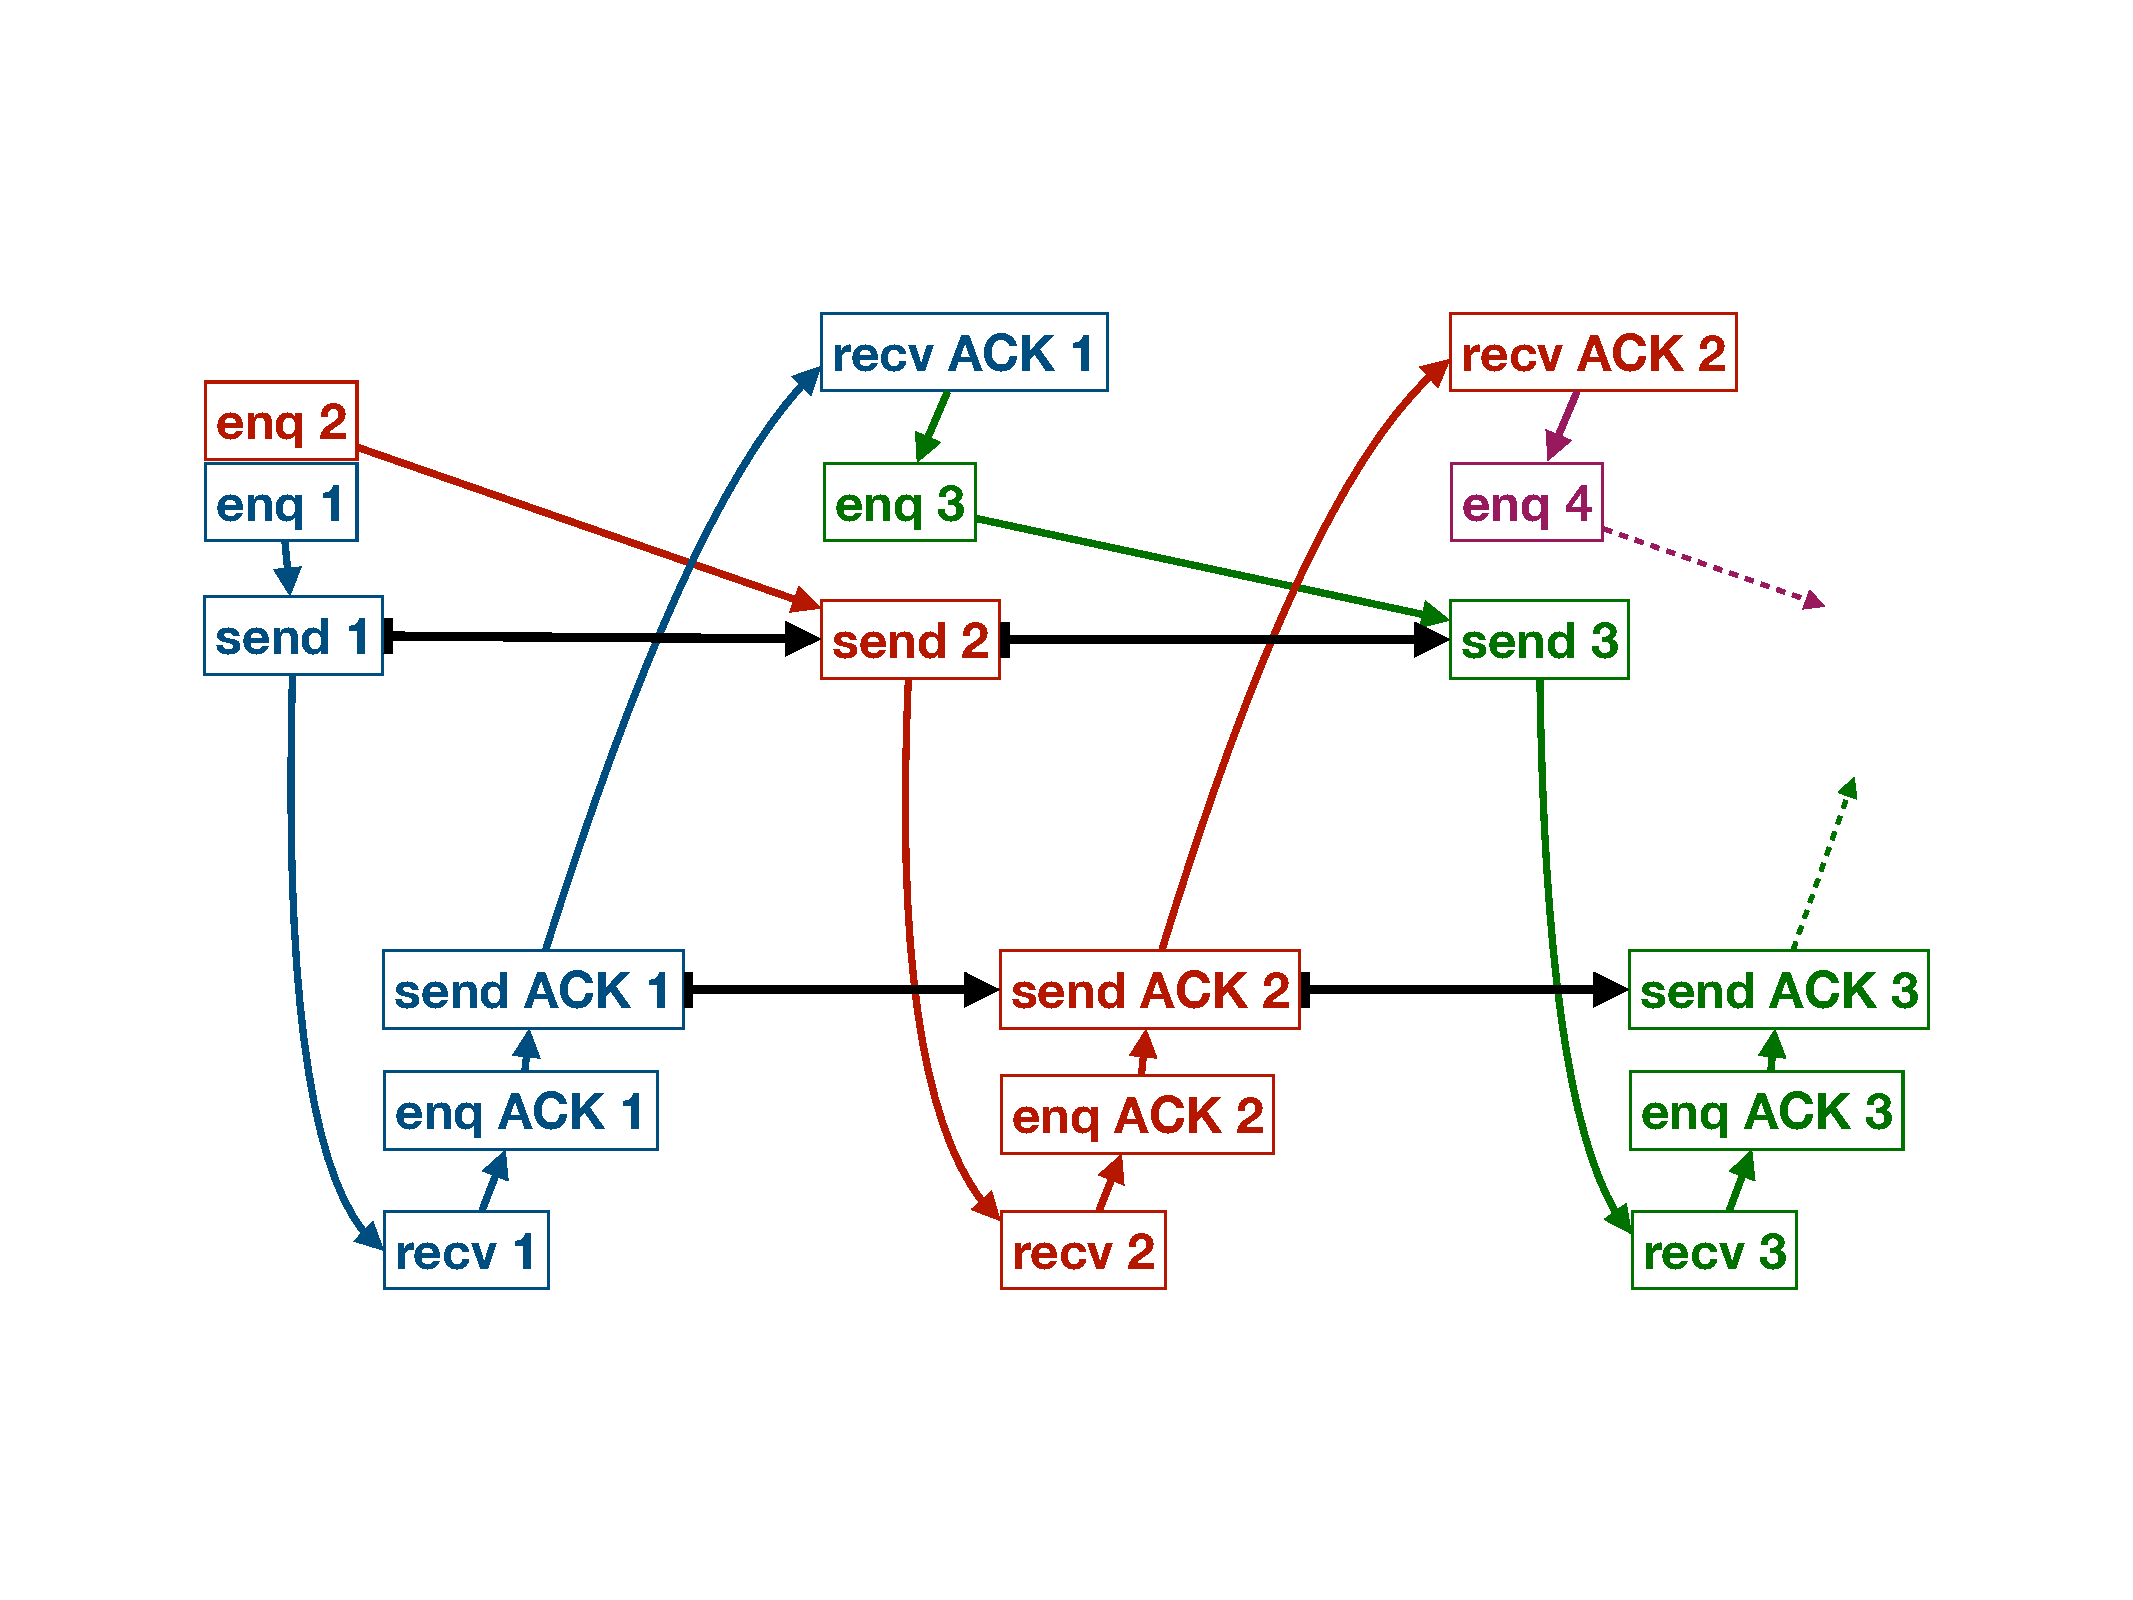
\includegraphics[width=\textwidth]{causality-concurrent}
        \caption{
            However, when the congestion window is larger, some events are independent from each other, for example \code{recv 1} and \code{send 2}. \manya{can you please high light these two events? shade the box or fill it with color.}
        }
        \label{causality-graph-para:fig}
    \end{subfigure}
    \caption{
        These two causality graphs are very similar, however, one permits concurrency and the other does not.
        Each graph corresponds to a sketch of a TCP exchange with a congestion window of 1 or 2.
        The arrows represent a direct dependency between two events, the black arrows between successive sends correspond to how long it takes to transmit a single packet.
        Every send implicitly depends on previous sends.
    }
    \label{causality-graph:fig}
\end{figure}

To better understand the opportunity, or lack thereof, for parallelization, it is necessary to better understand what causality requirements are imposed by the model.
A useful tool for this job is a causality graph \cite{misra_distributed_1986}.
A causality graph consists of a node for each event in the simulation, and a directed edge between from a dependency to the future event.
Any topological sort of the resulting graph is a valid execution order of the events.
Since the direction of the graph is always to the future, sorting the events by time is trivially correct.
This is the approach taken by the centralized simulator.

If a pair of events are direct ancestors/descendants of each other, i.e. there is a direct line going from one to the other, then there is a dependence between each other and they may not be executed simultaneously.
Conversely, if there is no direct connection between two events, they may be executed simultaneously.
This does not prevent events from sharing a common ancestor or descendant.

These events that are neither ancestor nor descendants are essentially independent of the current event, they can happen before, or after, or simultaneously, it will not affect the correctness of the simulation.
This is very similar to events outside the light-cone in physics \manya{cite}: events outside the light cone cannot have a causal relationship with the current point.
The correctness guarantee can therefore be reduced to knowing whether the next event to process has had all of its ancestors have been processed, i.e. it is safe.

A natural way to exploit concurrency in models is to run all the actors simultaneously \cite{misra_distributed_1986}.
From this actor-centric point of view, the concurrency guarantee is equivalent to processing events in order.
This means that an actor should only process an event if it is guaranteed that no other event will be received that would come before it.
This guarantee can be achieved if we require all actors to send each other events in order, a requirement many models already satisfy, and a common assumption \cite{fujimoto_parallel_2001}. 
In the rare case where this requirement isn't satisfied, it is usually possible to reformulate the model to comply with it.
We will see an example of such a reformulation when in section \ref{sim-timeouts} when we talk about timeouts.

An old algorithm, described as early as 1979\cite{fujimoto_parallel_2000}\cite{misra_distributed_1986} \manya{multiple citations are done with one \cite{X, Y}  command. please fix.}, is able to take these multiple in-order streams and safely return the next event.
Although taking the next event amongst all those received clearly is necessary to returning the next event, that alone is not sufficient.
For example, if the current next event would be scheduled at time 10, but we still haven't heard from a neighbour, we may later receive an event to be scheduled at time 9 from that neighbour, violating causality.
In order to avoid this situation, it is only safe to return an event when we have heard from \emph{every} neighbour. \manya{number 10 here is random, to make it more scientific, say time $t$.}

There exists a small relaxation of this strict requirement for events to be scheduled at the same time.
If we have already scheduled an event at time 10, we already know that no events will be scheduled before 10.
Therefore it is also safe to return all events that also happen exactly at time 10, even if we haven't heard from all our neighbours.
A common term for this time is \emph{safe time}, all events at or before the safe time are safe to schedule.
This handling of ties will turn out to be an important optimization when we talk about scheduling in section \ref{rustasim-sched}.


\subsection{Guaranteed progress with null-message passing} \label{null-messages}

Unfortunately, the algorithm above does not guarantee progress \cite{misra_distributed_1986}.
For example, in a network simulation where there are no packets to send, actors will not be sending any events to each other.
This will lead to every actor waiting on each other, leaving the simulation deadlocked.
These deadlocking patterns can be much more complex than two neighbours waiting on each other, and may involve a long ring of actors waiting on each other.
This problem is called distributed deadlock \cite{misra_distributed_1986}.

In order to overcome distributed deadlock, a new type of event is introduced: the null event.\manya{is this something you came up with or is this part of prior work? if this is your contribution, change the language from passive to active and move this to the next chapter. if this is from prior work, give citation.}
A null event is an event that represents the absence of event.
It is necessary because an actor cannot, on its own, distinguish between a lack of events due to another actor taking a long time and a lack of progress due to another actor not having any events to send.
Null events make it so that those cases can be distinguished: the presence of a null event signals that we can keep making progress, assured that we will not be receiving any more events from this actor before the null event.
A lack of events altogether implies that the actor has not been able to make progress yet.

A first, and technically correct, approach is to send null events to all of our neighbours after we process every event, including null events.
This does guarantee progress, however, since every null event causes every actor to send many new null events, this leads to an exponential growth of null events.
In order to mitigate this, actors can be made to only send null events to actors who have not yet heard from them at the current time.
Details of both these algorithms can also be seen in \cite{misra_distributed_1986}.

However, this approach of continuously sending null events can dramatically increase the number of events being sent.
Even though null events are fast to process, in some simulations, they can outnumber the number of non-null event 10 to 1 or more.
The algorithm I have gone for \manya{please use formal scientific language. this reads informal.} is a demand-based: null-events are only sent when we are unable to make progress otherwise.
If correctly implemented, this can result in some runs never requiring a single null event be sent.

When the simulator detects that there are no more safe events it declares a \emph{stall} and forces the actor to send a null message to all neighbours who need one.
A neighbour needs a null event if the last event we sent it was sent before the current safe time.
This might seem like an odd stipulation: by the nature of safe time, isn't it true that we will not have sent any neighour an event past the safe time?
However, that is often not true: actors might now \manya{know?} far ahead of time what they will be sending each other, in such a case, it is not necessary to send null events, the events we sent are enough to let them progress on their own.

Further optimization exist for null messages, for example \cite{wang_enhanced_2016} proposes null-message squashing and various loop optimizations.
The loop optimizations are very similar to the stall technique described above.

\manya{high-level comment: this subsection is a mix of what you had done and prior techniques. it would be good to separate these. the background section should only discuss prior work. you can give forward pointer to your approach but there is no need to discuss it here. Just talk about the challenges that prior work create and that your thesis addresses them in sections X and Y.}

\subsection{Other approaches}

Although the process described above \manya{please clarify exactly what you mean. the term "above" applies to everything you said in the thesis so far and the reader may not know exactly what process you are referring to.} is what I will be implementing in this thesis, other options exists for parallel discrete-event simulators.
Two are worth highlighting, both sacrifice accuracy in some way in order to obtain better performance.
The difference between the two approaches comes down to whether that accuracy error gets resolved or no.

\paragraph{Optimistic scheduling} \label{optimistic-scheduling}
It is also possible to allow actors to process events as fast as they can, possibly resulting in causality violations.
In order to maintain correctness, the simulation needs to have a cancellation mechanism, some use anti-events, checkpointing, rollbacks, or other techniques \cite{fujimoto_parallel_2015}.
This hopeful approach is the source of its name. \manya{any data center simulators using this?}

The cost of optimistic scheduling comes from the overhead necessary to allow for rollbacks, and the execution of these rollbacks.
\emph{TimeWarp} \cite{jefferson_virtual_1985} is a popular example of an optimistic scheduling algorithm.

Trying and rolling back is a common technique in computer engineering.
Databases use optimistic concurrency control instead of locks to rollback transactions in case of a conflict \cite{dragojevic_no_2015}.
CPUs are continuously predicting the next instruction to allow for higher speeds, but also need a cancelling mechanism if the prediction turns out incorrect.

Although correct, I have not explored this strategy out of a belief that it requires too much additional book-keeping to be useful.
This assumption has proven to be correct, on similar models, my simulator performs better than state of the art optimistic simulators. \manya{please quantify exactly how much better and in what sitation.}

However, optimistic simulators are able to make progress in models that the null-message passing algorithm cannot.
A null-message passing strategy relies on there being latency between actors, allowing them to make progress with respect to each other.
However, if the model asks for actors that may send each other events with no intervening delay, conservative simulators can get stuck: progress cannot be made if neither actor knows whether to expect an event from the other.
% mention rarely used small latency?
There are often ways to restructure the model in order to eliminate this situation, but this type of scenario is where optimistic strategies shine.

\paragraph{Loss of accuracy}
Another strategy could be to let execute events in the wrong order, possible yielding incorrect results. \manya{any papers that do this? cite them.}
Indeed, in an accurate simulator, incorrect results can result from an incorrect model or an incorrect simulator.
However, when giving up accuracy, the model may be correct, and properly implemented, but the results may still be off due to an unlucky run or a simulator bias.
Fundamentally, this makes trusting the results of the simulator harder.
In this thesis, correctness is an important design goal since it eliminates a source of errors, and I thus do not explore this strategy.
